%%%%
%       _  _____  ___  _____  _   _  ___ 
%      / \|_   _||_ _||_   _|| | | |/ __|
%     / △ \ | |   | |   | |  | |_| |\__ \
%    /_/¯\_\|_|  |___|  |_|   \___/ |___/
%                 EDUCAÇÃO
%    Modelo de TCC - Ciência da Computação
%%%%

\documentclass[12pt]{article}


\usepackage{graphicx, url}
\usepackage[utf8x]{inputenc}
\usepackage[french]{babel}
\usepackage[T1]{fontenc}
\usepackage[english=american]{csquotes}
\usepackage{float}
\usepackage{comment}
\usepackage{amsmath}
\usepackage{amssymb}
\usepackage{enumerate}
\usepackage{subcaption}
\usepackage{setspace}
\usepackage{tabularray}

\usepackage[style=abnt]{biblatex}

% indica o arquivo com as referencis bibliograficas
\addbibresource{}

\title{Optimisation du moment et de la fréquence d'injection de traitement pour les gliomes de bas grades chez l'adulte} % titulo

\author{Maia COLLIN, Paul HENTON, Ambre JAEGER} % autor principal, orientador

\usepackage{fancyhdr}
\usepackage{geometry}
\usepackage{hyperref}
\usepackage{color} 
\hypersetup{
unicode=true,
pdfauthor={},
pdfkeywords={},
pdftitle={},
pdfsubject={},
pdfstartview={FitV}, 
    colorlinks,%
    citecolor=blue,%
    filecolor=blue,%
    linkcolor=red,%
    urlcolor=blue
}

\geometry{hmargin=2cm, vmargin=2cm }

\pagestyle{fancy}
\fancyhf{}
\rfoot{}
\lhead{\textbf{\large TP Modélisation  - M2 2024}}
\rhead{\textbf{\large M. Collin, P. Henton, A. Jaeger}}


% %%%%%%%%%%%%%%%%%%%%%%%%%%%%%%%%%%%%%%%%%%%%%%%%%%%%%%%%%%%%%%

\begin{document}
\maketitle % Não remova essa linha!
     
\section{Introduction}
Que sont les gliomes de bas-grades leurs propriétés ?\\
Quels sont les traitements existants?\\
Question scientifiques: \textbf{Quels sont les temps et fréquences optimales d'administration du traitement pour maximiser leur efficacité ?}


\section{Etude du modèle}
tgtbtbvhtb dcsdc sdc q
\subsection{Présentation du modèle}
\begin{figure}
    \centering
    \begin{subfigure}[t]{0.45\textwidth}
        \centering
        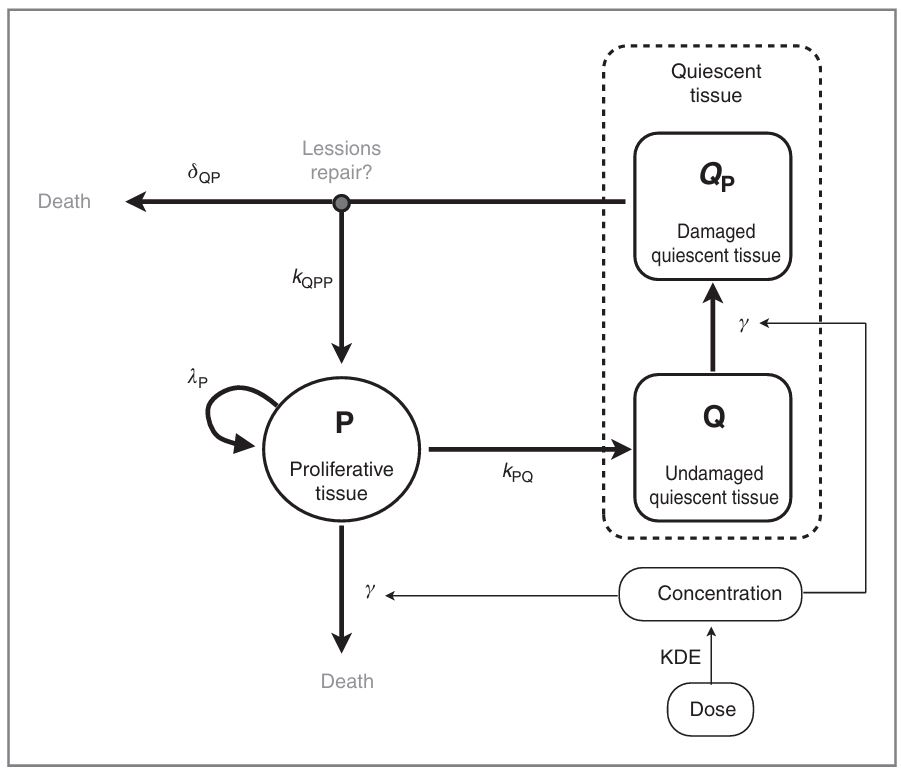
\includegraphics[width=\linewidth]{Image/modele.JPG} 
        \caption{} \label{fig:model}
    \end{subfigure}
    \hfill
    \begin{subfigure}[t]{0.45\textwidth}
        \centering
        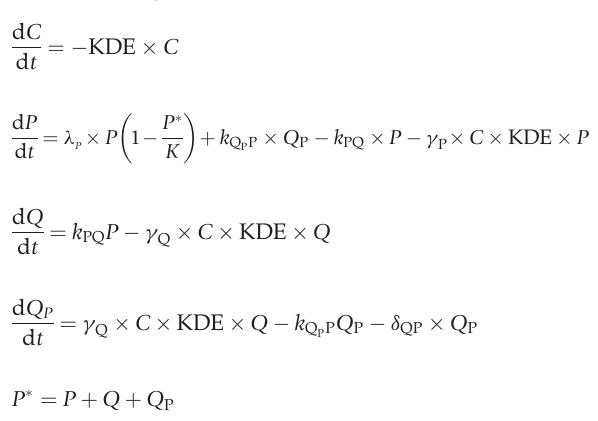
\includegraphics[width=\linewidth]{Image/eq.JPG} 
        \caption{} \label{fig:teq}
    \end{subfigure}

     \vspace{1cm}
    \begin{subfigure}[t]{\textwidth}
    \centering
        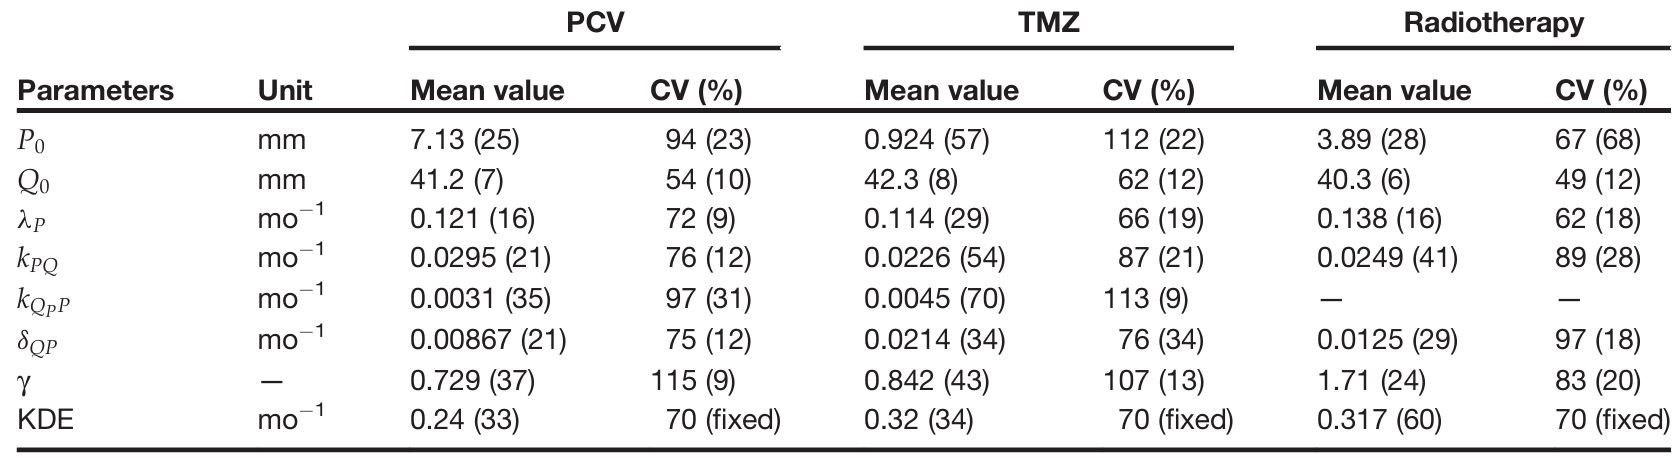
\includegraphics[width=\linewidth]{Image/tableau.JPG} 
        \caption{} \label{fig:tableau}
    \end{subfigure}
    
    \caption{\textbf{Présentation du modèle \cite{} (a).} Modèle à 3 compartiments $P$ (tissu prolifératif), $Q$ (tissu quiescent), $Q_{p}$ (tissu quiescent endommagé). Sous l'effet du traitement de concentration C (normalisée) qui va endommagé l'ADN des cellules, P peut être endommagé et mourir selon efficacité $\gamma$ et Q peut devenir $Q_p$ selon efficacité $\gamma$. $Q_{p}$ mourrir selon $\delta$ ou redevenir prolifératif. Les coefficients $k$ désigne la proprtion de tissu qui transitionne vers un autre état.  \textbf{(b).} Mise en équation du modèle proposé. \textbf{(c).} Estimation des paramètres d'après fitting de données de patients ayant subi les différents traitements au modèle. CV désigne le coefficient de variation qui caractérise la variabilité interindividuelle. L'erreur sur les estimations est donnée par les nombres entre parenthèses en pourcentage. Pour plus de précisions se référer à l'article référence\cite{}}
\end{figure}


\begin{figure}
    \centering
    \begin{subfigure}[t]{0.45\textwidth}
        \centering
        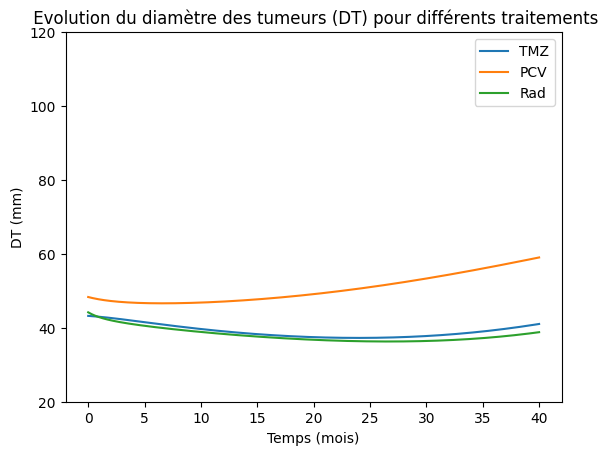
\includegraphics[width=\linewidth]{Image/evolution_TD_param_moy.png} 
        \caption{} \label{fig:timing1}
    \end{subfigure}
    \hfill
    \begin{subfigure}[t]{0.45\textwidth}
        \centering
        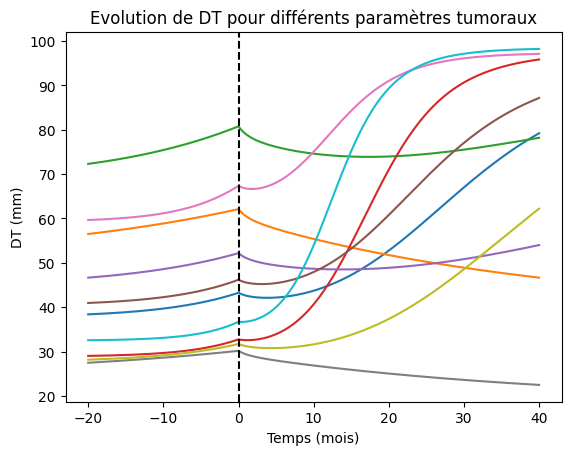
\includegraphics[width=\linewidth]{Image/ex_traj.png} 
        \caption{} \label{fig:timing2}
    \end{subfigure}

    \caption{\textbf{(a).} Evolution du diamètre d'une tumeur (DT) pour les paramètres de populations moyens des trois traitements chimio thérapie PCV, TMZ ou radiothérapie \cite{}. \textbf{(b).} Evolution du DT pour les paramètres moyens PCV sauf $\lambda_{p}$, $P_{0}$, $Q_{0}$ choisi aléatoirement selon les distributions les valeurs moyennes et coefficient de variation indiqué dans \ref{} }
\end{figure}

\subsection{Exploration de l'espace des paramètres}

\begin{figure}
    \centering
    \begin{subfigure}[t]{0.45\textwidth}
        \centering
        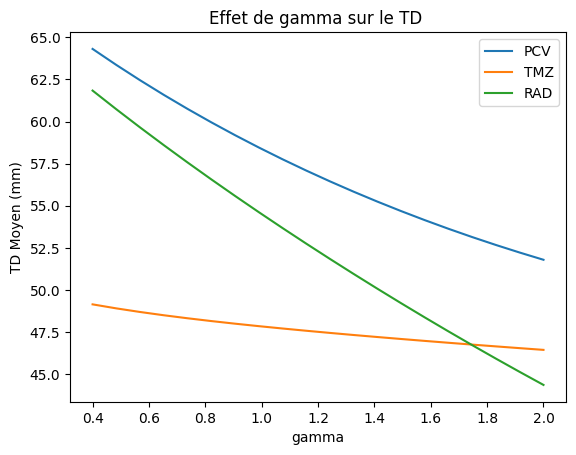
\includegraphics[width=\linewidth]{Image/effet_gamma.png} 
        \caption{} \label{fig:effet_C}
    \end{subfigure}
    \hfill
    \begin{subfigure}[t]{0.45\textwidth}
        \centering
        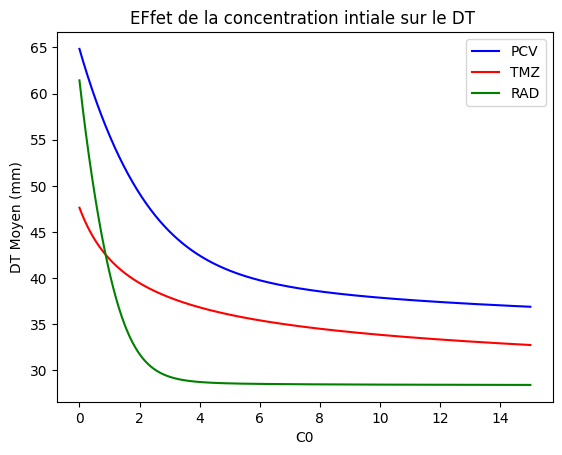
\includegraphics[width=\linewidth]{Image/effet_C.png} 
        \caption{} \label{fig:effet_gamma}
    \end{subfigure}

    \caption{\textbf{(a).} Effet de $\gamma$ sur le DT, les autres paramètres sont choisis selon les valeurs moyennes des traitements. \textbf{(b).} Effet de $C$ sur le DT, les autres paramètres sont choisis selon les valeurs moyennes des traitements.}
\end{figure}

\section{Optimisation du moment et de la fréquence d'injection}
\subsection{Optimisation pour une unique injection}

\section{Conclusion}
\subsection{Limites}
\subsection{Perspectives}


% %%%%%%%%%%%%%%%%%%%%%%%%%%%%%%%%%%%%%%%%%%%%%%%%%%%%%%%%%%%%%%
% Seção de Referências (gerada automaticamente)
\printbibliography  % Não remover esta linha
% %%%%%%%%%%%%%%%%%%%%%%%%%%%%%%%%%%%%%%%%%%%%%%%%%%%%%%%%%%%%%%

\end{document}